\documentclass[ExampleMasters.tex]{subfiles}
\begin{document}

	\chapter{APPENDIX B}
	{\Large Driving Cycle Synthesis}

	\section{Data analysis and fitting}

	The aim of the project is to find the most productive vehicle combination for a particular route. The route chosen for this is the 294 km E20/E6 highway from G\"oteborg to Malm\"o. This particular journey back and forth is quite popular among companies transporting goods and any findings of the report will be of key interest. 
	The driving cycle data provided was recorded with a frequency of 1 Hz from an on-board GPS and it included:
	\begin{itemize}
		\item X-axis position data
		\item Y-axis position data
		\item Z-axis position data
		\item Velocity
		\item Distance covered
	\end{itemize}

	The inputs that are required from the driving cycle are the information of road gradient, instantaneous velocity and acceleration. Each of which could have been directly used from the provided data. However on subsequent study the speed signal was found to have considerable noise and many data points missing, making it unusable. The distance signal did not correspond to the distance covered as calculated from the position signal according to the equation below.

	\begin{equation} \label{eq:cycle distance}
	Distance = \sqrt{(x_{i+1} - x_i)^2 +(y_{i+1} - y_i)^2}
	\end{equation}

	This left only the position signals which had some issues that posed problems at first. The data is used to obtain the values of the slope of the road along the z axis (? Road gradient) since the vehicle model is represented as a one-track bicycle model and lateral effects are neglected. This is done as 

	\begin{equation} \label{eq:cycle slope}
	Slope =\frac{\delta Height}{\delta Distance} = \frac{z_{i+1} - z_i}{\sqrt{(x_{i+1}-x_i)^2 +(y_{i+1}-y_i)^2  }}
	\end{equation}

	The resolution of the position data was determined to be too low which caused problems when the slope was calculated as there were sudden big jumps in the slope values.

	\begin{figure}[hb]
		\begin{center}
			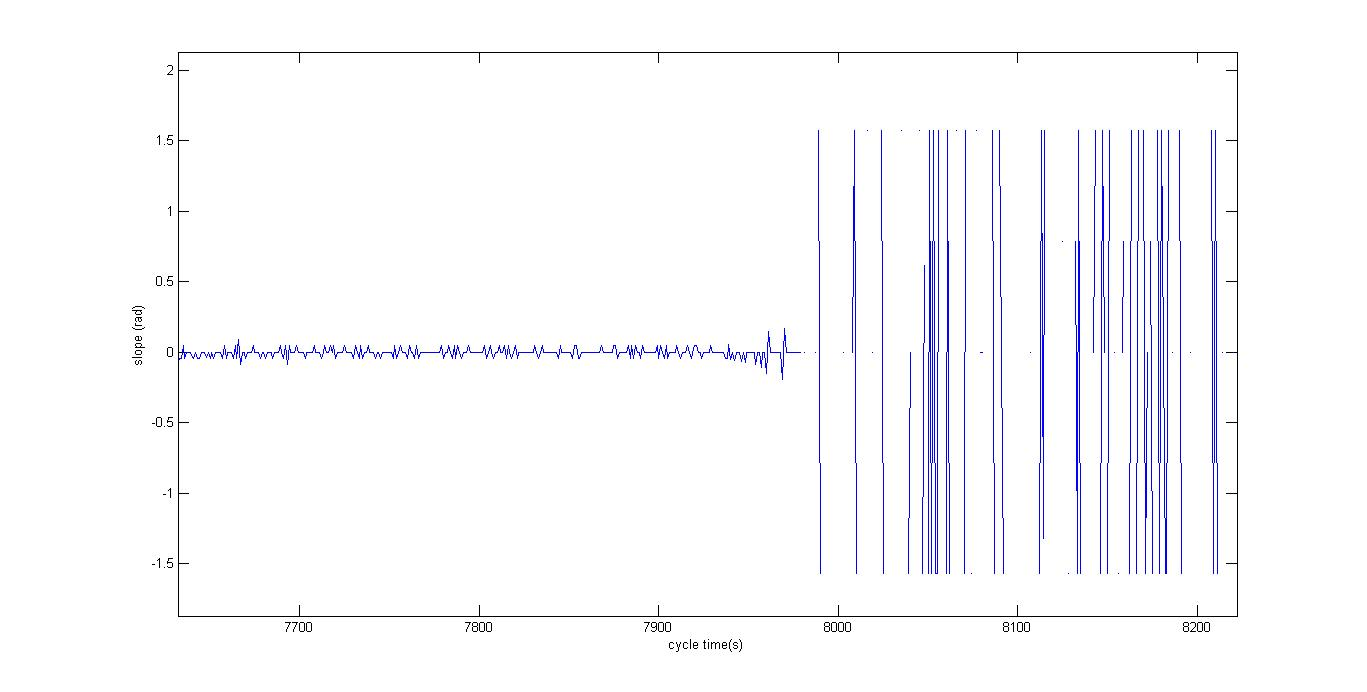
\includegraphics[width=0.75\textwidth]{figures/VehicleModel/noise.pdf}
		\end{center}
		\caption{Noisy slope signal.}
		\label{fig:noise}
	\end{figure}

	The data was also inconsistent resulting in a much disrupted slope signal as can be seen in figure (\ref{fig:noise}).This was addressed by introducing a rolling average filter for the position data along each axis. This approximates the value of the position over a range of old data to the average value in that range. The size of the range is dependent on the speed of the truck (i.e. taking a small sample size when the truck is moving faster and vice-versa) in order to provide a more realistic new signal. The sampling range was 10 above a threshold speed of 40 kmph and 5 for speeds below. When the position signals were filtered the slope was recalculated using equation (\ref{eq:cycle slope}). This gave an improved new slope data (data 2) as shown in figure(\ref{fig:rollingavg}).

	\begin{figure}
		\begin{center}
			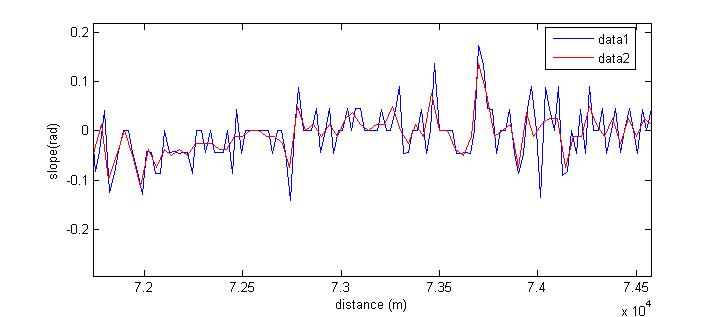
\includegraphics[width=0.75\textwidth]{figures/VehicleModel/rollingavg.pdf}
		\end{center}
		\caption{Slope signal after rolling average.}
		\label{fig:rollingavg}
	\end{figure}

	While the slope signal was now less irregular with a sampling frequency of 1 Hz the calculated slope was still too noisy to be used directly. To ensure the signal was smoother, a Matlab cubic spline function was used with a tuning factor of 0.1.Lastly the slope signal was redefined as against distance rather than time to suit the functionality of the driver model which is explained in more detail in Section  \ref{sec:drivermodel}.

	\begin{figure}
		\begin{center}
			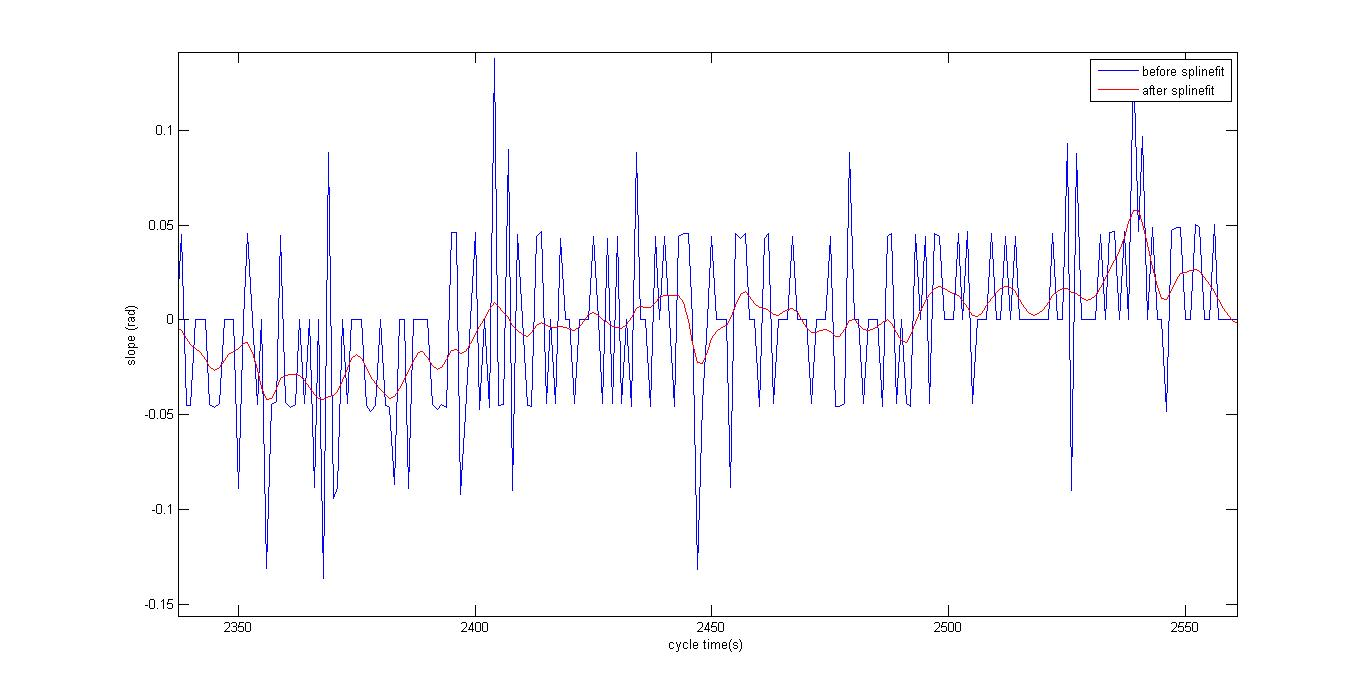
\includegraphics[width=0.75\textwidth]{figures/VehicleModel/aftersplinefit.pdf}
		\end{center}
		\caption{Slope signal after splinefit.}
		\label{fig:aftersplinefit}
	\end{figure}

	\newpage

\end{document}